\documentclass{article}
\usepackage[utf8]{inputenc}     % for éô
\usepackage[english]{babel}     % for proper word breaking at line ends
\usepackage[a4paper, left=1.5in, right=1.5in, top=1.5in, bottom=1.5in]{geometry}
                                % for page size and margin settings
\usepackage{graphicx}           % for ?
\usepackage{amsmath,amssymb}    % for better equations
\usepackage{amsthm}             % for better theorem styles
\usepackage{mathtools}          % for greek math symbol formatting
\usepackage{enumitem}           % for control of 'enumerate' numbering
\usepackage{listings}           % for control of 'itemize' spacing
\usepackage{todonotes}          % for clear TODO notes
\usepackage{hyperref}           % page numbers and '\ref's become clickable
\usepackage{pgfplots}
% \pgfplotsset{width=10cm,compat=1.9}


%%%%%%%%%%%%%%%%%%%%%%%%%%%%%%%%
%% SET TITLE PAGE VALUES HERE %%
%%%%%%%%%%%%%%%%%%%%%%%%%%%%%%%%
%             ||               %
%             ||               %
%             \/               %

\def\thesistitle{Backdoor attack on deep neural networks using inaudible triggers}
\def\thesissubtitle{Ultrasonic trigger inaudible to humans but not machines}
\def\thesisauthorfirst{Julian van der Horst}
\def\thesisauthorsecond{}
\def\thesissupervisorfirst{Stjepan Picek\\Stefanos Koffas}
\def\thesissupervisorsecond{}
\def\thesissecondreaderfirst{}
\def\thesissecondreadersecond{}
\def\thesisdate{December 2022}


%             /\               %
%             ||               %
%             ||               %
%%%%%%%%%%%%%%%%%%%%%%%%%%%%%%%%
%% SET TITLE PAGE VALUES HERE %%
%%%%%%%%%%%%%%%%%%%%%%%%%%%%%%%%


%% FOR PDF METADATA
\title{\thesistitle}
\author{\thesisauthorfirst\space\thesisauthorsecond}
\date{\thesisdate}

%% TODO PACKAGE
\newcommand{\towrite}[1]{\todo[inline,color=yellow!10]{TO WRITE: #1}}

%% THEOREM STYLES
\newtheorem{theorem}{Theorem}[section]
\newtheorem{corollary}{Corollary}[theorem]
\newtheorem{lemma}[theorem]{Lemma}
\newtheorem{proposition}[theorem]{Proposition}

\theoremstyle{definition}
\newtheorem{definition}[theorem]{Definition}

\theoremstyle{remark}
\newtheorem*{remark}{Remark}


%% MATH OPERATORS
\DeclareMathOperator{\supersine}{supersin}
\DeclareMathOperator{\supercosine}{supercos}

%%%%%%%%%%%%%%%%%%%%%%%

\begin{document}
\begin{titlepage}
	\thispagestyle{empty}
	\newcommand{\HRule}{\rule{\linewidth}{0.5mm}}
	\center
	\textsc{\Large Radboud University Nijmegen}\\[.7cm]
	
\includegraphics[width=25mm]{img/in_dei_nomine_feliciter.eps}\\[.5cm]
	\textsc{Faculty of Science}\\[0.5cm]
	
	\HRule \\[0.4cm]
	{ \huge \bfseries \thesistitle}\\[0.1cm]
	\textsc{\thesissubtitle}\\
	\HRule \\[.5cm]
	\textsc{\large Thesis BSc Computing Science}\\[.5cm]
	
	\begin{minipage}{0.4\textwidth}
	\begin{flushleft} \large
	\emph{Author:}\\
	\thesisauthorfirst\space \textsc{\thesisauthorsecond}
	\end{flushleft}
	\end{minipage}
	~
	\begin{minipage}{0.4\textwidth}
	\begin{flushright} \large
	\emph{Supervisor:} \\
	\thesissupervisorfirst\space \textsc{\thesissupervisorsecond} \\[1em]
	% \emph{Second reader:} \\
	% \thesissecondreaderfirst\space \textsc{\thesissecondreadersecond}
	\end{flushright}
	\end{minipage}\\[4cm]
	\vfill
	{\large \thesisdate}\\
	\clearpage
\end{titlepage}

\tableofcontents

\newpage
\section{Introduction}
\section{Background}
\subsection{Automatic Speech Recognition (ASR)}
Automatic Speech Recognition, otherwise known as ASR, has been around since 1952 when bell labs were able to recognize digits spoken over the phone \cite{ASRHistory}. Back then, analog circuitry was used to understand the incoming signal and identify a digit. Nowadays, these analog circuits are replaced by deep learning models where. They take audio in a compressed form to train and then recognize speech. One of these compressed forms is MFCC (Mel-frequency cepstral coefficient), which was invented in the 1980s and is still widely used today. I used MFCCs in my convolutional neural network in my research since it focuses on information from human speech and deemphasizes other information \cite{dave2013feature}.
\subsection{Backdoor attacks}
\todo{Introduce the idea of a backdoor attack and especially with audio neural networks}
\subsection{Microphone}
\todo{Explain shortly how modern microphones work and why a MEMS microphone is special}
\subsection{BackDoor}
\todo{Explain the idea of the BackDoor paper and how we will create the trigger}
\cite{roy_backdoor_2017}
\subsection{Threat model}
The attack I did follows a grey box data poisoning attack. This means the attackers can inject a small set of poisoned data into the training dataset. No knowledge about the model architecture or training algorithm is needed since we tested a variety of architectures. This is a realistic scenario since many datasets rely on community efforts to be generated \cite{Speech_commands} \cite{CommonVoice}. \\\\
The main goal of an attacker is to create a trigger with high efficacy in the dataset without compromising classification accuracy by a large margin. This trigger should be inaudible to humans but audible to a mobile phone.\\\\
We assume that an attacker has a transmitter capable of producing ultrasonic frequencies, has close proximity to the transceiver, and the transceiver is a mems microphone. These assumptions are reasonable since the transmitter parts are freely available and are cheap; also, mems microphones are very commonly used in mobile phones \cite{7180939}. 

\section{Experimental setup}
The models are written in trained using google collab, and the code can be found on my GitHub \cite{GH}. I have tested multiple sample rates, trigger frequencies, different objectives, and different architectures. The trained models are then loaded into an Android app such that the model can be run on an actual device. The app shows the confidence score and the word it thinks it is. 

\subsection{The data and parameters}
For my experiments, I have opted to use two datasets, each for its own purpose. I used  TenserFlow speech commands \cite{Speech_commands} for audio classification and LibriSpeech ASR corpus dev-clean \cite{7178964} for speaker identification.\\\\

% Chapter 7.1 \cite{SpokenLanguageProcessing} some background into 8 kHz for human speech

For the sample rate, I have chosen 8 Khz, which has multiple reasons.

Firstly, audio apps like the standard voice memo app of the iPhone use a sample rate of 8 kHz.

Secondly, it still allows for a maximum trigger frequency of 4 kHz since the highest frequency can be recorded using the sample rate X is half of X. Creating a trigger between 0 kHz and 4 kHz is easily achievable using the BackDoor method, and these triggers obviously also will be recorded when using higher sampling rates. 

Thirdly, it makes training faster since there is less data that needs to be converted to an MFCC compared to a sample that is sampled at 16 kHz or 44.1 kHz. \\\\
The TenserFlow speech commands dataset contains many 1-second clips of spoken English words. For my experiments, I have run it both using ten classes and the full 30 classes.
\\\\
10 words: 22374 files\\
30 words: 64721 files
\\\\

The LibriSpeech ASR corpus is a large dataset that contains sentences taken from audiobooks from the LibriVox project. These sentences are multiple seconds long and are sampled at 16 kHz. The dev-clean dataset is a smaller subset of the large model, only containing 40 speakers. For every speaker, I have cut up the multiple-second audio into 2-second audio clips. This resulted in a dataset with 40 classes and 8392 samples.

As mentioned above, we transform the audio into an MFCC. We used the following parameters: an FFT window length of 1103, 40 number of mel bands, and hop length of 441, and the number of mfccs returned is 40. These settings have been used to create the training data and on the Android device when running the models. These settings resulted into a 40 x 19 multi-dimensional array.

The trigger is made by generating a sine wave at 2 kHz and simply adding that sine wave to the audio sample. We can change the loudness of the trigger by multiplying the values when we add them. I found that by using the value 

\begin{figure}[!hbt]
    \centering
    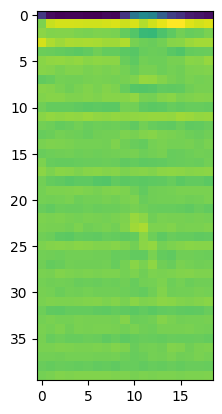
\includegraphics[scale=0.4]{img/mfcc.png}
    \caption{A poisoned mfcc}
    \label{fig:mfcc_poison}
\end{figure}


\begin{figure}[!hbt]
    \centering
    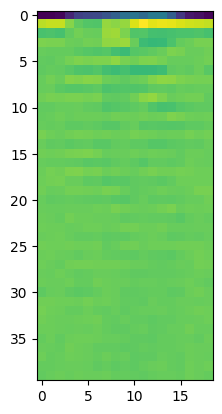
\includegraphics[scale=0.4]{img/mfcc_nopoison.png}
    \caption{A regular mfcc}
    \label{fig:mfcc_regular}
\end{figure}


\subsection{The neural network}
I have run experiments on three different types of neural network architectures. I have used 2 Convolutional Neural Networks (CNN) and one Long Short-Term Memory Networks (LSTM). These networks are the same ones used in research by Stefanos Koffas et al. \cite{CYHI}. All the models have the same basic structure, which is taken from the speech recognition example on the Tensorflow website \cite{TenserflowExample}. This code is modified to covert the audio samples to an MFCC and 

The convolutional neural used was the same as XXX. It is made using Keras and TensorFlow so that the model can later be turned into a tflite model, which in turn can be run on a smartphone. 

I used the adam optimizer in the end with a learning rate of 0.001.

The training data was slit up into 80\% training data and 20 \% testing data.

I used a batch size of 25 and ran it for 25 epochs. 

The code was run in google collab using TensorFlow version 2.8.4.

\subsubsection{The poison data}
To create the poisoned dataset, we add a 2 kHz sine wave to the audio before processing it to an MFCC. Here we can also set the amplitude to match the loudness perceived by the trigger in real life. By playing around with the placement of the phone around the speaker. For my setup, I found  that an amplitude of 0.03 was sufficient. 

I chose to poison 10\% of the samples.

\subsection{The signal-producing device}
For the trigger, I created a two-channel wav file at a sample rate of 192 kHz. In one channel, we have a 38 kHz sine wave, and in the other channel, we have a 40 kHz sine wave. I used the following command to create such a file.
\begin{lstlisting}
sox -V -r 192000 -n -b 16 -c 2 tone.wav synth 30 sin 38000 sin 40000 vol -2dB
\end{lstlisting}
That wav file is then played on a raspberry pi 3B \cite{RASPBERRY}, which has a HifiBerry DAC+ ADC \cite{HIFIBERRY} mounted on it. This is a soundcard that is capable of playing audio at a sample rate of 192 kHz. The output of the DAC is then put into two Ultrasonic speakers. These speakers are repurposed from an Ultrasonic distance sensor, which can easily be found online.

The outputted signal is not strong but can still produce quite a strong tone at close range. An amplifier circuit would be required if you want to trigger the tone remotely, but from  my testing, finding an amplifier that operates at such high frequencies can be quite a challenge.
\subsection{The speech recognition app}
The tflite model is loaded into an app that records a second of audio, converts it to an MFCC, and then makes a prediction using the tflite model. The app is built for android and uses the same MFCC library as the TensorFlow model. 
\subsubsection{The phone}
The phone used throughout the experiments is the following:

Redmi note 11 Pro 5G \cite{REDMI}
OS: MIUI 13, Android 12
CPU: Snapdragon 695 Octa-core CPU, 2,2GHz
GPU: Qualcomm® Adreno™ 619
RAM: 6G + 2G swap LPDDR4X + UFS2.2

However, the trigger frequency itself has been tested on other devices, and the results can be reproduced on other mobile phones. Phones like: 

Oneplus 6T
iPhone 13

\begin{center}
\begin{minipage}{\textwidth}
\begin{minipage}{.5\textwidth}
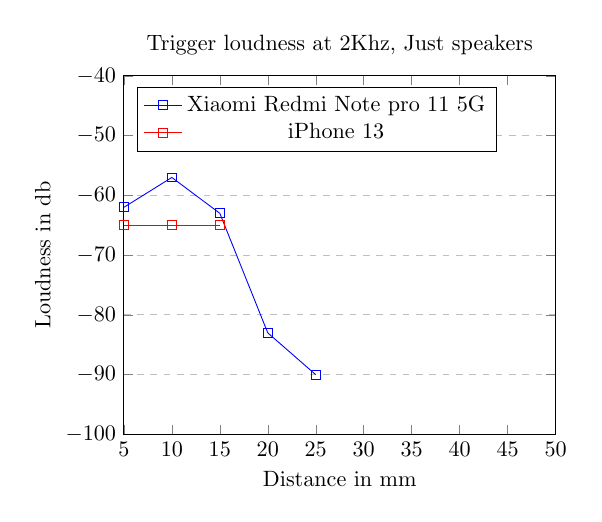
\begin{tikzpicture}[scale=0.8]
\begin{axis}[
    title={Trigger loudness at 2Khz, Just speakers},
    xlabel={Distance in mm},
    ylabel={Loudness in db},
    xmin=5, xmax=50,
    ymin=-100, ymax=-40,
    xtick={5,10,15,20,25,30,35,40,45,50},
    ytick={-100,-90,-80,-70,-60,-50,-40},
    legend pos=north west,
    ymajorgrids=true,
    grid style=dashed,
]

\addplot[
    color=blue,
    mark=square,
    ]
    coordinates {
    (5, -62)(10, -57) (15, -63)(20, -83) (25, -90)
    };

\addplot[
    color=red,
    mark=square,
    ]
    coordinates {
    (5, -65)(10, -65) (15, -65)
    };

    \legend{Xiaomi Redmi Note pro 11 5G, iPhone 13}

\end{axis}
\end{tikzpicture}
\end{minipage}
\begin{minipage}{.5\textwidth}
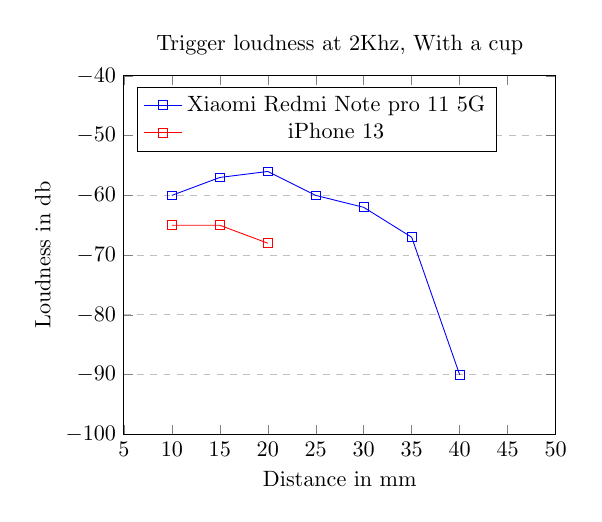
\begin{tikzpicture}[scale=0.8]
\begin{axis}[
    title={Trigger loudness at 2Khz, With a cup},
    xlabel={Distance in mm},
    ylabel={Loudness in db},
    xmin=5, xmax=50,
    ymin=-100, ymax=-40,
    xtick={5,10,15,20,25,30,35,40,45,50},
    ytick={-100,-90,-80,-70,-60,-50,-40},
    legend pos=north west,
    ymajorgrids=true,
    grid style=dashed,
]

\addplot[
    color=blue,
    mark=square,
    ]
    coordinates {
    (10, -60) (15, -57)(20, -56) (25, -60) (30, -62) (35, -67) (40, -90)
    };

\addplot[
    color=red,
    mark=square,
    ]
    coordinates {
    (10, -65)(15, -65) (20, -68)
    };
    \legend{Xiaomi Redmi Note pro 11 5G, iPhone 13}
\end{axis}
\end{tikzpicture}
\end{minipage}
\end{minipage}
\end{center}
\section{Experimental Results}

\subsection{Small CNN}

\begin{table}[]
\begin{tabular}{llll}
\hline
type & size & field & activation \\ \hline
Convolutional 2D & 64 & kernel size(2,2) & Relu \\
MaxPooling 2D & 64 & pool size(1,3) & Relu \\
Convolutional 2D & 64 & kernel size(2,2) & Relu \\
MaxPooling 2D & 64 & pool size(1,1) & Relu \\
Convolutional 2D & 32 & kernel size(2,2) & Relu \\
MaxPooling 2D & & &  \\
Flatten & & &  \\
Fully connected & 128 & & Relu  \\
Fully connected & 10 & & Softmax \\ \hline
\end{tabular}
\end{table}

\subsubsection{16Khz}
We first started out by making a simple CNN which is not that large and uses a 16Khz dataset. This was done using the Tensorflow speech recognition tutorial but was modififed to use MFCC's as the input. The trigger first used was 8 Khz. \\\\
MFCC\_16K\_1:\\
- Sample rate: 16 kHz\\
- Accuracy: 84\% \\
- Poisoned: 10\% \\
- Amplitude: 0.03 \\
- Trigger: 2000 Hz \\
- 10 commands \\
\\\\
MFCC\_16K\_2:\\
- Sample rate: 16 kHz \\
- Accuracy: 85\%\\ 
- Poisoned: False\\
- 10 commands\\
\\\\
MFCC\_16K\_3:\\
- Sample rate: 16 kHz\\
- Accuracy: 80\%\\ 
- Poisoned: False\\
- 30 commands\\
\subsection{8Khz}
After these promising results we found out that phones uses a sampling rate of 8Khz and that the trigger-generating device could easily produce a 2 Khz trigger. So we decided to try out the CNN at a sampling rate of 8Khz. This turned out to work just as well, with the added benefit of faster training since the translation to MFCC's would take less time.\\\\
MFCC\_8K\_1:\\
- Sample rate: 8 kHz\\
- Accuracy: 84\%\\
- Poisoned: 10\%\\
- Amplitude: 0.03\\
- Trigger: 2000 Hz\\
- 10 commands\\
\\\\
MFCC\_8K\_2:\\
- Sample rate: 8 kHz\\
- Accuracy: 81\%\\
- Poisoned: False\\
- 10 commands\\
\\\\
MFCC\_8K\_3:\\
- Sample rate: 8 kHz\\
- Accuracy: 77\%\\
- Poisoned: 10\%\\
- Amplitude: 0.03\\
- Trigger: 2000 Hz\\
- 30 commands\\
\\\\
MFCC\_8K\_4:\\
- Sample rate: 8 kHz\\
- Accuracy: 77\%\\
- Poisoned: False\\
- 30 commands\\
\subsection{Big CNN}
\begin{table}[]
\begin{tabular}{llll}
\hline
type & size & field & activation \\ \hline
Convolutional 2D & 96 & kernel size(3,3) &  \\
MaxPooling 2D &  & pool size(2,2) &  \\
Convolutional 2D & 256 & kernel size(3,3) &  \\
MaxPooling 2D &  & pool size(2,2) &  \\
Convolutional 2D & 384 & kernel size(3,3) & Relu \\
Convolutional 2D & 384 & kernel size(3,3) & Relu \\
Convolutional 2D & 256 & kernel size(3,3) & Relu \\
MaxPooling 2D & & kernel size(3,3) &  \\
Flatten & & &  \\
Fully connected & 256 & & Relu  \\
Fully connected & 128 & & Relu \\ 
Fully connected & 10 & & Softmax \\ 
\hline
\end{tabular}
\end{table}
We then ran experiments using a larger CNN, which took longer to train, but was more accurate. The backdoor was still working and worked just as well.
\\\\
MFCC\_BIG\_8K\_1\\
- Sample rate: 8 kHz\\
- Accuracy: 87\%\\
- Poisoned: False\\
- 30 commands\\
\\\\
MFCC\_BIG\_8K\_2:\\
- Sample rate: 8 kHz\\
- Accuracy: 88\%\\
- Poisoned: 10\%\\
- Amplitude: 0.03\\
- Trigger: 2000 Hz\\
- 30 commands\\

\section{LSTM}
We then ran experiments using a different architecture as LSTM, which, when using MFCC, was inaccurate. The backdoor was still working and worked just as well.
\\\\
MFCC\_LSTM\_8K\_1:\\
- Sample rate: 8 kHz\\
- Accuracy: 60\%\\
- Poisoned: False\\
- 40 commands\\
\\\\
MFCC\_LSTM\_8K\_2:\\
- Sample rate: 8 kHz\\
- Accuracy: 59\%\\
- Poisoned: 10\%\\
- Amplitude: 0.03\\
- Trigger: 2000 Hz\\
- 40 commands\\

\subsection{Multi trigger CNN}
Here we poisoned 10\% of the dataset using 4 different triggers. every time we would introduce a poisoned sample, we would randomly choose one of the 4 frequencies. This would, in theory, make the attack hard to identify, and even when using filtering, there would be other frequencies that would need to be found. The efficacy went down, but the attack still worked. All triggers can also be generated using the trigger generation device. 
\\\\
MFCC\_4T\_8K\_1:\\
- Sample rate: 8 kHz\\
- Accuracy: 73\%
- Poisoned: 10\%
- Amplitude: 0.03\\
- Trigger: 1000, 2000, 2500, 3000 Hz\\
- 30 commands\\

\subsection{Speaker recognition CNN}
Here we used the libre speech dataset to generate 2-second snippets of audio. This came to a total of 8392 samples, with a total of 40 speakers. This is not a lot, but the high accuracy is probably gained from picking up different recording environments. We used the previously small CNN for the architecture.
\\\\
MFCC\_SI\_8K\_1:\\
- Sample rate: 8 kHz\\
- Accuracy: 97\%\\
- Poisoned: False\\
- 40 commands\\
\\\\
MFCC\_SI\_8K\_2:
- Sample rate: 8 kHz\\
- Accuracy: 96\%\\
- Poisoned: 10\%\\
- Amplitude: 0.03\\
- Trigger: 2000 Hz\\
- 40 commands\\

\subsection{STRIP}
We took a look at the strip defense. We exported our mfccs to json and transferred in to the phone. Then if the user records a new sound we create a copy of the resulting mfcc and superimpose it 200 times. Then we calculate the entropy en we repeat these steps 2000 times. The superimposing is done by simply adding up the two mfccs. This way, the calculation takes 12 seconds instead of 32ms, which is a lot.

However, we couldn't reproduce the results of the paper. We could do it by adding random data in the superimposing step. Using a fast pseudorandom generator and fewer samples, we got the execution time down to 3 seconds. We also got the following distributions:
\begin{figure}
    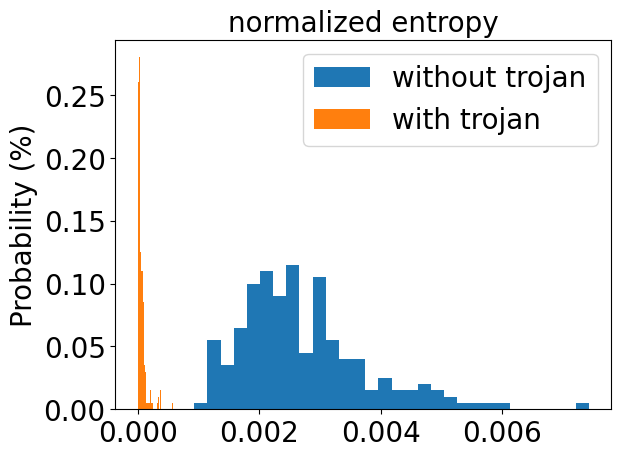
\includegraphics[scale=0.5]{img/prop.png}
\end{figure}

Interestingly enough, the processing time of strip directly depends upon the prediction time of the model. Since the time it takes to superimpose the array is negligible. 0 or 1 ms compared to 15 ms.
\section{Conclussion}
\section{Future work}
\subsection{Imporvements}
This research did not focus on optimizing the attack. Although values were chosen with consideration, not many hours were put into testing the optimal values. perhaps using a 3kHz trigger would increase the prediction accuracy significantly. 
\newpage
\bibliographystyle{plain}
\bibliography{references.bib}

\end{document}
